\section{Auswertung}
\label{sec:Auswertung}

Die Messwerte welche im ersten Teil des Experiments aufgenommen wurden sind in Tabelle \ref{tab:doppler} zu finden.
Dafür wurde die Frequenz des reflektierten Schalls unter Variation des Einstellwinkels und der Umdrehungsgeschwindigkeit gemessen.
Die verwendete Pumpe lies keine direkte Einstellung der Fließgeschwindigkeit zu.
Stattdessen wird als Maß die Umdrehungen pro Minute der Pumpe ($rpm$) verwendet.

\begin{table}
    \centering
    \begin{tabular}{ccc}
    \toprule
    $\text{Prismenwinkel}/\SI{}{\degree}$ & $N/rpm$ &  $\nu_\text{g}/\SI{}{\Hz}$ \\
    \midrule
    15 & 2020 & 78      \\
    15 & 3000 & 145     \\
    15 & 4050 & 220     \\
    15 & 6050 & 520     \\
    15 & 5000 & 390     \\
    30 & 2020 & 95      \\
    30 & 3000 & 224     \\
    30 & 4050 & 375     \\
    30 & 5000 & 655     \\
    30 & 6050 & 884     \\
    45 & 2020 & 144     \\
    45 & 3000 & 360     \\
    45 & 4050 & 630     \\
    45 & 6050 & 1520    \\
    45 & 5000 & 1090    \\
    \bottomrule
    \end{tabular}
    \caption{Die gemessenen Frequenzen in Abhängigkeit des Prismenwinkel und der Umdrehungen pro Minute der Pumpe.}
    \label{tab:doppler}
\end{table}

Das Verhältnis $\frac{\nu_\text{g}}{\cos \alpha}$ ist in Abbildung \ref{fig:doppler} graphisch gegen die Umdrehungsgeschwindigkeit der Pumpe aufgetragen.
Alle Plots wurden mit dem Python-Paket matplotlib \cite{matplotlib} erstellt.

\begin{figure}
    \centering
    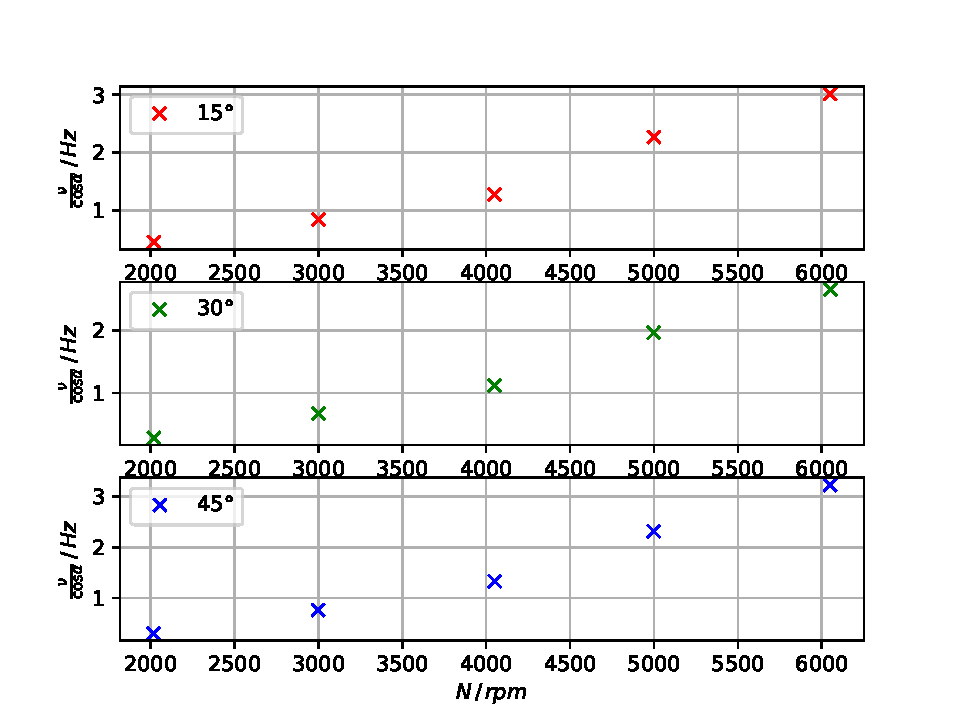
\includegraphics[width=\textwidth]{content/data/doppler.pdf}
    \caption{Die aufgenommenen Frequenzen aufgetragen gegen die Umdrehungsgeschwindigkeit der Pumpe.}
    \label{fig:doppler}
\end{figure}

\FloatBarrier

Im nächsten Teil des Experiments wurde die Streuintensität $I$ sowie die maximale Frequenz $f_\text{max}$ des reflektierten Schalls in Abhängigkeit der Messtiefe der Schallsonde gemessen.
Dafür wurden an der Sonde verschiedene Messtiefen in $\si{\micro\second}$ eingestellt.
Die so aufgenommenen Werte sind in Tabelle \ref{tab:depth} zu finden.
In dem linken Teil der Tabelle sind dabei die Messwerte für eine Umdrehungsgeschwindigkeit von $N = \SI{3880}{rpm}$ zu sehen und im rechtem Teil der Tabelle die Messwerte für $N = \SI{6000}{rpm}$.

\begin{table}
    \centering
    \begin{tabular}[t]{ccc}
    \toprule
    $Tiefe \,/\, \SI{}{\micro\second}$ & $I \,/\, \SI{}{100\frac{\volt^2}{\second}} $ & $f_\text{max}\,/\, \SI{}{\Hz} $\\
    12.5 & 93 & 400     \\
    13.0 & 130 & 430    \\
    13.5 & 200 & 500    \\
    14.0 & 207 & 502    \\
    14.5 & 215 & 514    \\
    15.0 & 160 & 490    \\
    15.5 & 160 & 457    \\
    16.0 & 300 & 420    \\
    16.5 & 301 & 380    \\
    17.0 & 190 & 400    \\
    17.5 & 155 & 400    \\
    18.0 & 184 & 390    \\
    18.5 & 196 & 400    \\
    19.0 & 225 & 430    \\
    \bottomrule
    \end{tabular}
    \begin{tabular}[t]{ccc}
    \toprule
    $Tiefe \,/\, \SI{}{\micro\second}$ & $I \,/\, \SI{}{100\frac{\volt ^2}{\second}} $ & $f_\text{max}\,/\, \SI{}{\Hz} $\\
    12.5 & 100 & 800        \\
    13.0 & 120 & 860        \\
    13.5 & 200 & 1020       \\
    14.0 & 235 & 1092       \\
    14.5 & 260 & 1185       \\
    15.0 & 350 & 1206       \\
    15.5 & 370 & 1225       \\
    16.0 & 400 & 1020       \\
    16.5 & 390 & 930        \\
    17.0 & 420 & 950        \\
    17.5 & 345 & 980        \\
    18.0 & 320 & 990        \\
    18.5 & 300 & 1100       \\
    19.0 & 260 & 1200       \\
    \bottomrule
    \end{tabular}
    \caption{Die Streuintensität und die maximale Frequenz des reflektierten Schalls in Abhängigkeit der Messtiefe. Die Messwerte der linken Tabelle wurden bei $N = \SI{3880}{rpm}$ gemessen, die der rechten bei $N = \SI{6000}{rpm}$}
    \label{tab:depth}
\end{table}

Für eine graphische Auftragung der Messwerte wird zunächst aus der Messtiefe $s$ in $\si{\micro\second}$ die Messtiefe in $\si{\milli\meter}$ berechnet.
Daür wird zunächst die Strecke $s_\text{prism}$ subtrahiert, die der Schall im Prisma zurücklegt.
\begin{equation*}
 s_\text{liquid} = s - \frac{s_\text{prism}}{c_\text{prism}}
\end{equation*}
$c_\text{prism}$ entspricht dabei der Schallgeschwindigkeit im Prisma.
Daraufhin wird mit dem Weg-Zeit-Gesetz
\begin{equation*}
l = c_\text{liquid} \cdot s,
\end{equation*}
die Messtiefe $s$, mithilfe der Schallgeschwindigkeit $c_\text{liquid}$ in der Flüssigkeit, in eine Distanz $l$ in $\si{\milli\meter}$ umgerechnet.
Gegen diese wird nun die Streuintensität $I$ und die maximale Frequenz $f_\text{max}$ graphisch aufgetragen.
Die graphisch aufgetragenen Messwerte sind für $N = \SI{3880}{rpm}$ in Abbildung \ref{fig:3880} und für $N = \SI{6000}{rpm}$ in Abbildung \ref{fig:6000} zu finden.

\begin{figure}
    \centering
    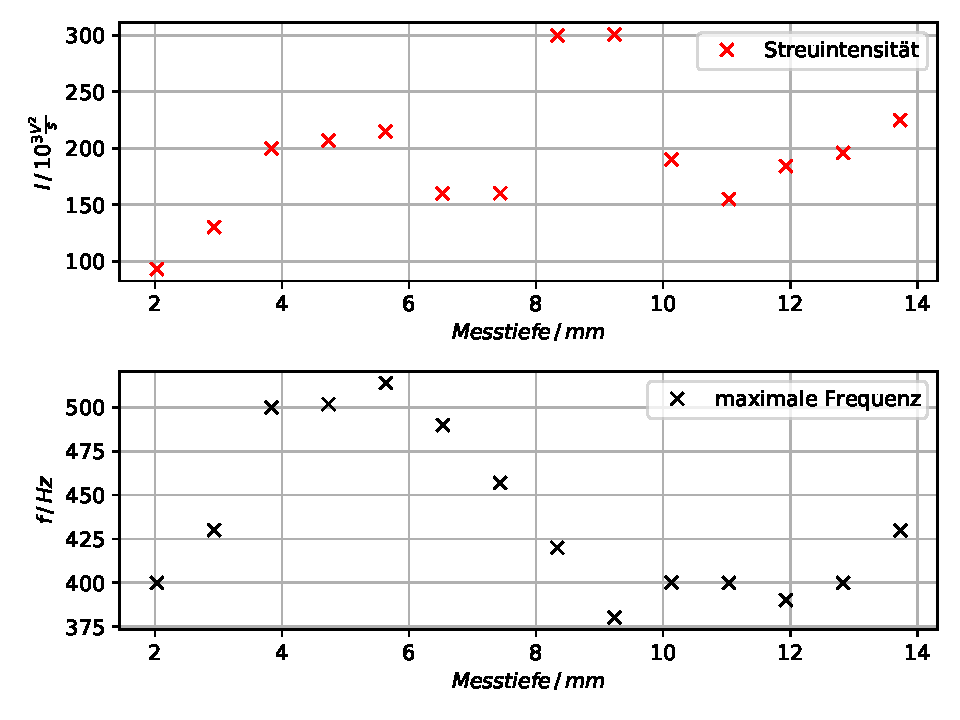
\includegraphics[width=\textwidth]{content/data/depth_3880.pdf}
    \caption{Die obere Graphik zeigt die Streuintensität aufgetragen gegen die Messtiefe, die untere die Frequenz aufgetragen gegen die Messtiefe. $N=\SI{3880}{rpm}$}
    \label{fig:3880}
\end{figure}

\begin{figure}
    \centering
    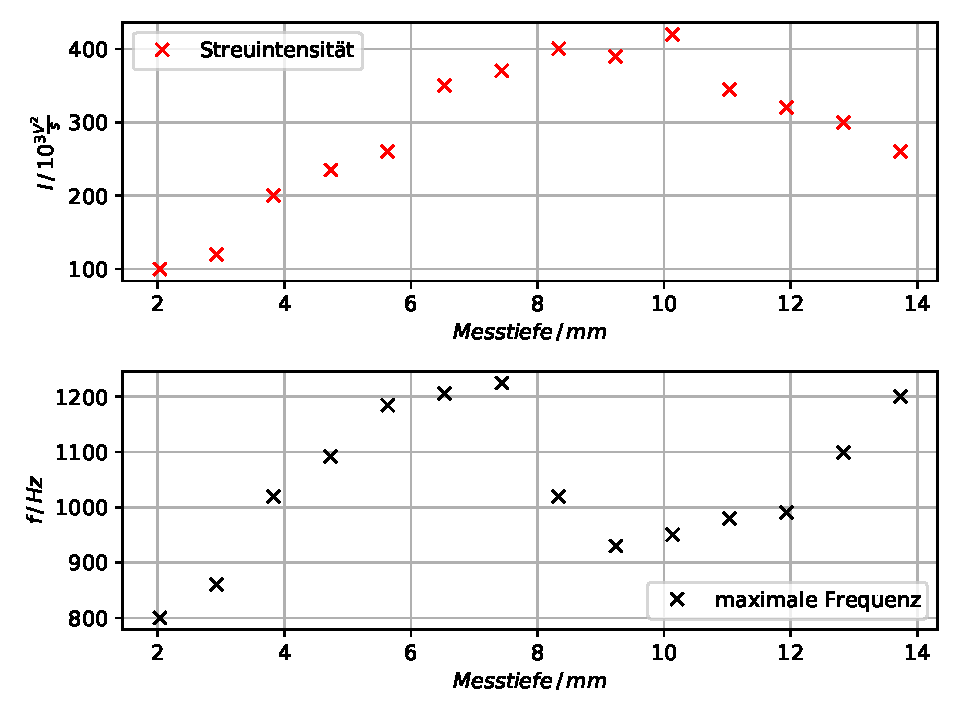
\includegraphics[width=\textwidth]{content/data/depth_6000.pdf}
    \caption{Die obere Graphik zeigt die Streuintensität aufgetragen gegen die Messtiefe, die untere die Frequenz aufgetragen gegen die Messtiefe. $N=\SI{6000}{rpm}$}
    \label{fig:6000}
\end{figure}
